% LaTeX formatting example for NERCCS
% Revised on 11/07/2020 by Dane Taylor

\documentclass[12pt]{article}
\usepackage[letterpaper,margin=1in]{geometry}
\usepackage{times}
\usepackage{graphicx}
\usepackage{sectsty}
\usepackage{setspace}
\usepackage{caption}
\allsectionsfont{\normalsize}
\usepackage{authblk}
\renewcommand\Authfont{\normalsize}
\usepackage{etoolbox}
\patchcmd{\thebibliography}{\section*{\refname}}{}{}{}

\let\OLDthebibliography\thebibliography
\renewcommand\thebibliography[1]{
  \OLDthebibliography{#1}
  \setlength{\parskip}{1pt}
  \setlength{\itemsep}{7pt plus 0.3ex}
}

\begin{document}

\title{\normalsize\bf \vspace{-10ex}
A Network Approach to Cancer: Clustering Cell Lines by Gene Dependency Rank Distances}

\begingroup\onehalfspacing
\author{Jane Adams$^1$, Celestin Coquide$^2$, Diana Garcia$^3$, Rodrigo Migueles Ramirez$^4$ \\
\footnotesize
$^1$ Vermont Complex Systems Center, University of Vermont, United States $^2$ Institut UTINAM, OSU THETA, University of Bourgogne, France, $^3$ National Institute of Genomics Medicine, Mexico City, Mexico,  $^4$ Quantitative Life Sciences Interfaculty Program, McGill University, Montreal, Canada }
\endgroup



\date{\vspace{-5ex}} % to kill the unnecessary blank space for \date{}

\maketitle

\thispagestyle{empty}
\pagestyle{empty}
Cancer heterogeneity is one of the main obstacles that prevent efficient treatment: each tumor is usually composed of widely divergent cells. Conversely, different types of cancer can present unexpected genetic similarities. Recently, the DepMap project \cite{Tsherniak17} evaluated the gene dependency for survival in cancer cell lines using CRISPr technology to target a wide number of genes (18k) with sgRNAs. In this project, we use the Achilles dataset from the DepMap project to find similarities between 625 different cancer cell lines based on their genetic dependency profiles. The genetic dependency profiles are characterized by a gene effect score and a gene dependency probability. Spearman’s rank correlation coefficients were calculated on the dependency probability matrix between each pair of cell lines. A backbone method  \cite{Serrano09} was applied to the correlation matrix resulting in a network with 12 connected components. Half of the components were composed of heterogeneous tumour origins, accounting for 84.21$\%$ of the cell lines. One prominent component containing 60 nodes from 12 different types of cell lines features pancreatic cancer as the central hub. Although some same origin cell line cliques, like leukemia cell lines, 93.75$\%$ of the cell lines have a tendency to be preferentially linked with cell lines of different origins, as measured by balanced homophily. These results suggest that this approach could allow us to identify genes to which cancer types are similarly vulnerable, thus providing hints for combinatorial therapies and novel applications for existing therapeutic strategies. 


\begin{figure}[h]
\centering
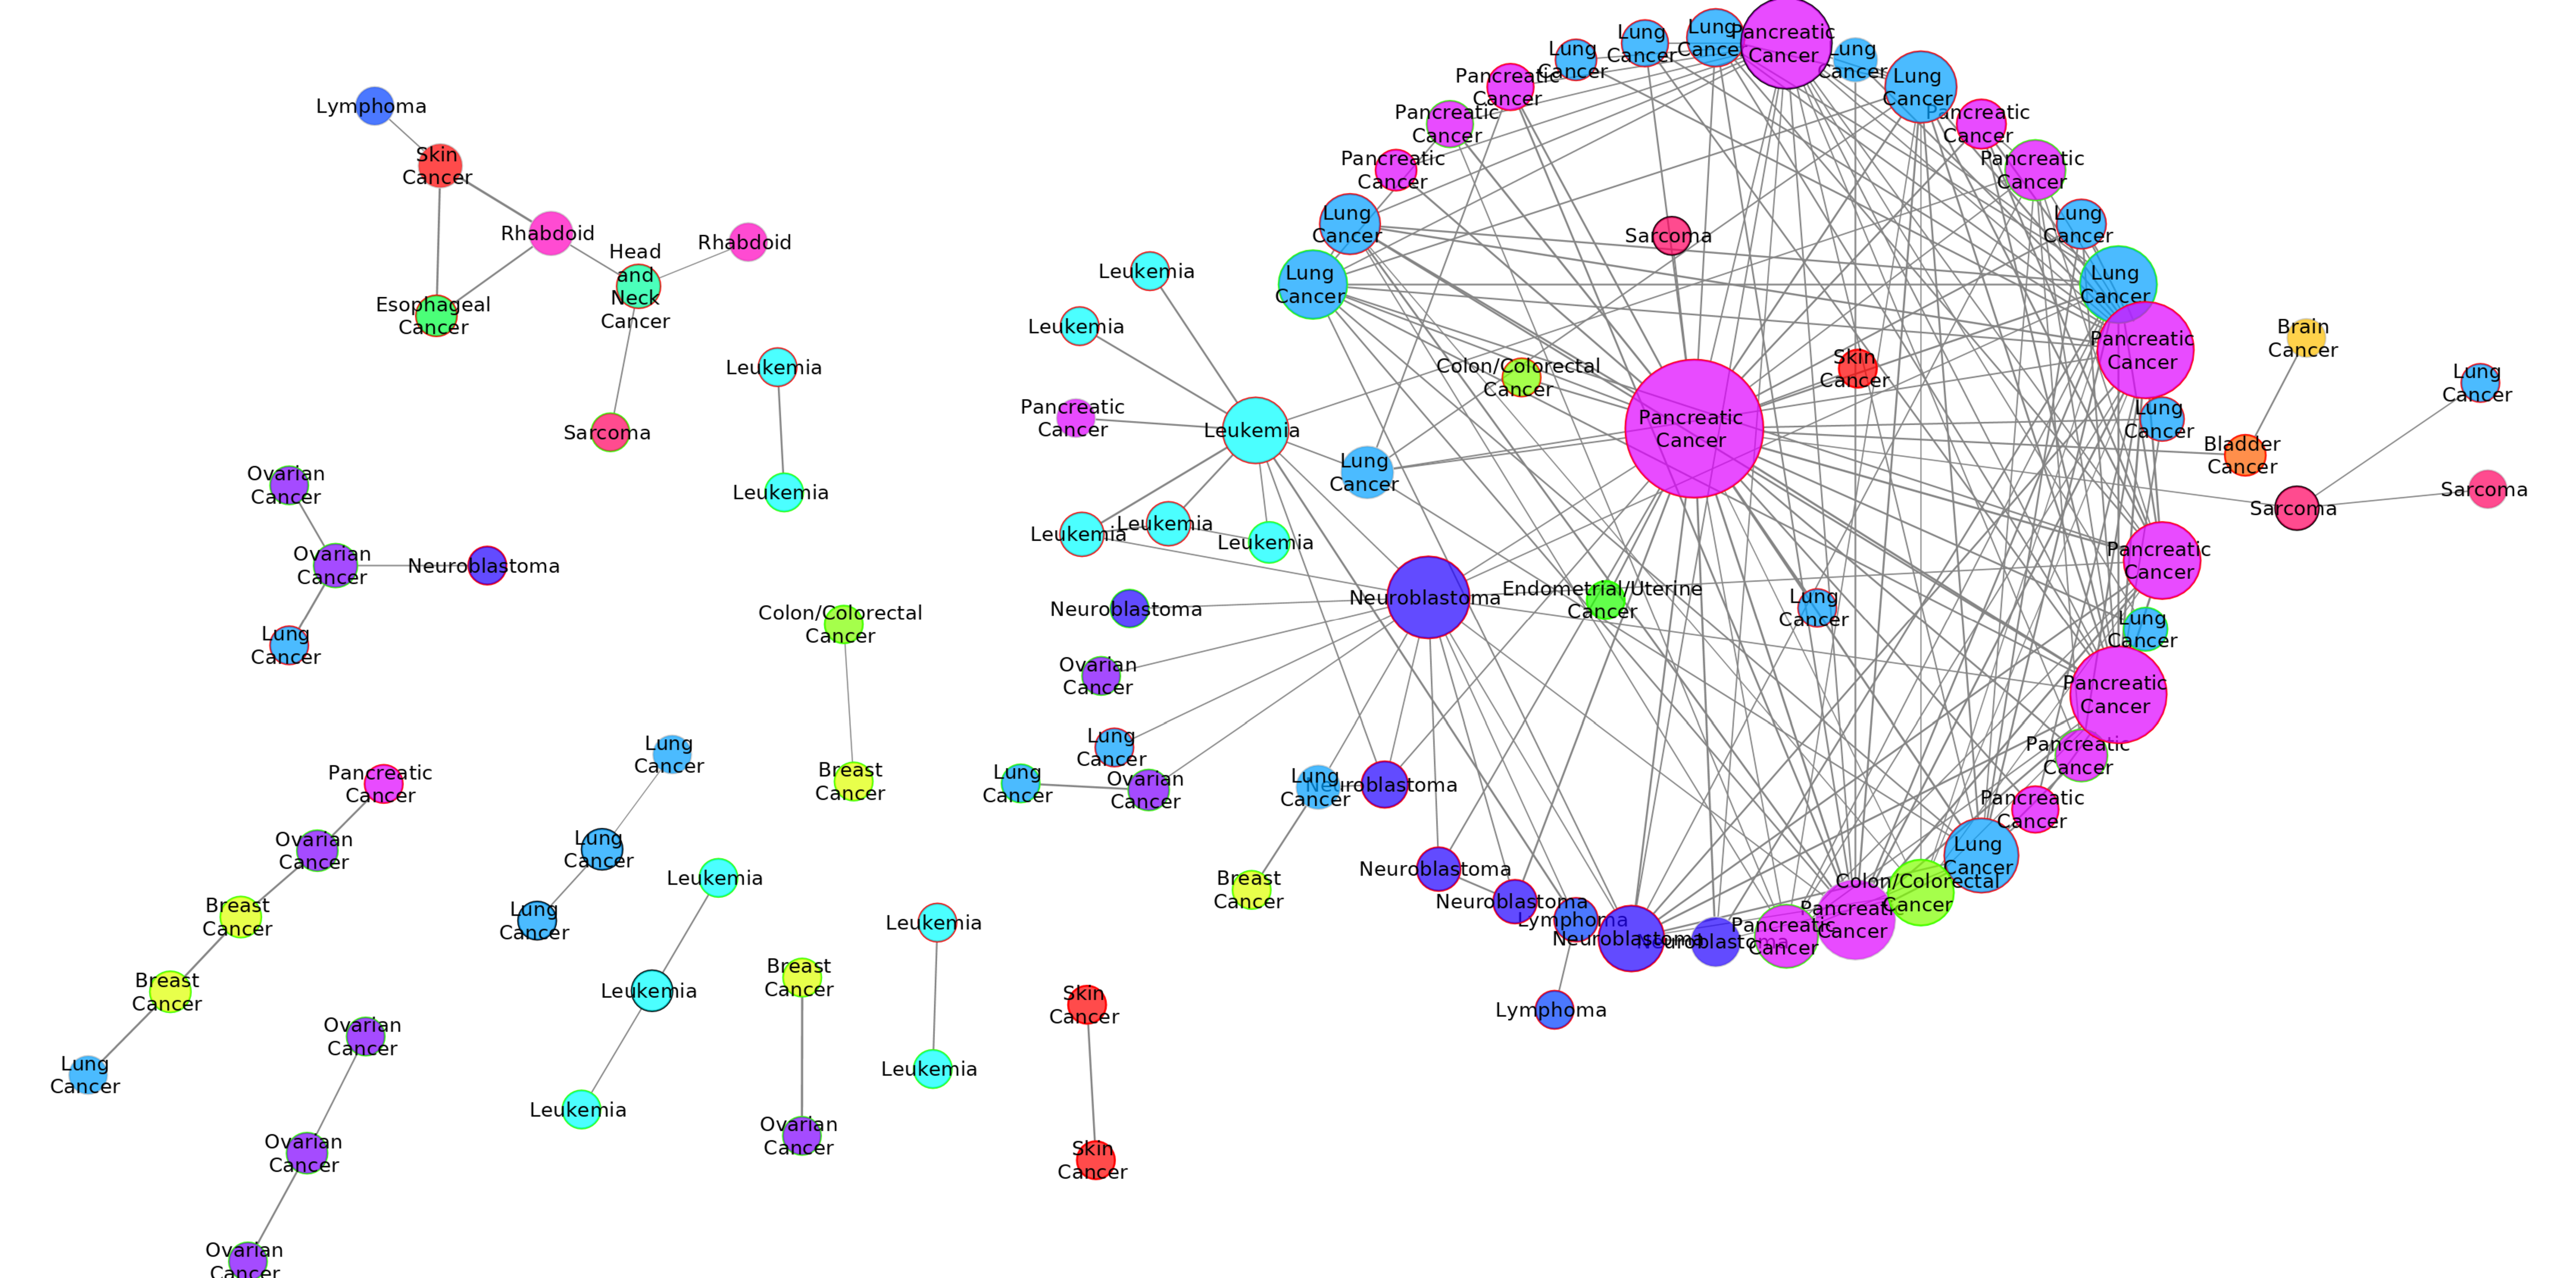
\includegraphics[width=1\columnwidth]{fig1.pdf} 
 \caption*{\scriptsize Network of cell-cell gene dependence similarities. Cell lines are colored according to their cancer type. A total of 95 cell lines and 213 links.}
\end{figure}


 
\begin{thebibliography}{99}
\vspace{-2ex}
\scriptsize
\bibitem{Tsherniak17} Tsherniak, A. et al. {\textit{Defining a Cancer Dependency Map.}} Cell 170, 564-576.e16 (2017). DOI: 10.1016/j.cell.2017.06.010.
\vspace{-2ex}
\bibitem{Serrano09} Serrano, M. et al. {\textit{Extracting the Multiscale Backbone of Complex Weighted Networks}}. Proceedings of the National Academy of Sciences Apr 2009, 106 (16) 6483-6488; DOI: 10.1073/pnas.0808904106

\end{thebibliography}

\end{document}